\documentclass[../main.tex]{subfiles}

\begin{document}
	\section{Sistema}
		\'E un oggetto (fisico/astratto) in cui si riescono a individuare diverse quantit\'a che variano nel tempo e tra le quali si pu\'o riconoscere una relazione causa-effetto.

	\subsection{Amplificatore ideale lineare}
		\begin{wrapfigure}{r}{0.5\linewidth}%
			\vspace{-40pt}
			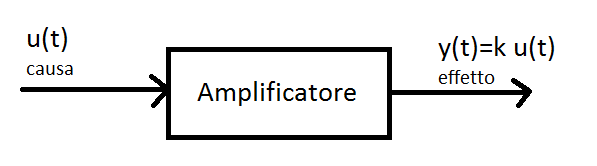
\includegraphics[width=\linewidth]{introduzione/amplificatore}
		\end{wrapfigure}
		L'amplificatore ideale \'e un sistema in cui l'uscita (effetto) $y(t)$ dipende linearmente dall'ingresso (causa) $u(t)$.
		
	\section{Sistema dinamico}
		\'E un sistema i cui effetti non dipendono unicamente dal valore istantaneo delle cause, ma possono dipendere dalla storia delle cause, dallo stato del sistema in un determinato momento, dalle condizioni iniziali.\\
		Il numero di condizioni iniziali determina l'ordine del sistema.
		
	\subsection{Circuito RC} 
		Consideriamo il circuito RC in figura dove $v_{in}$ \'e la causa e $v_{out}$ \'e l'effetto.
		\begin{figure}[H]
			\centering
			\begin{circuitikz} \draw
				(0,0)	to[V, v=$ v_{in} $] (0,3)
						to[short](1,3)
						to[R, l_=$ r $, v^<=$ v_R $](3,3)
						to[short, i=$ i $](4,3)
						to[C, l_=$ C $, v^<=$ v_1 $](4,0)
						to[short](0,0)
				;
			\end{circuitikz}
			\begin{subfigure}{0.48\linewidth}
				\vspace{-2cm}
				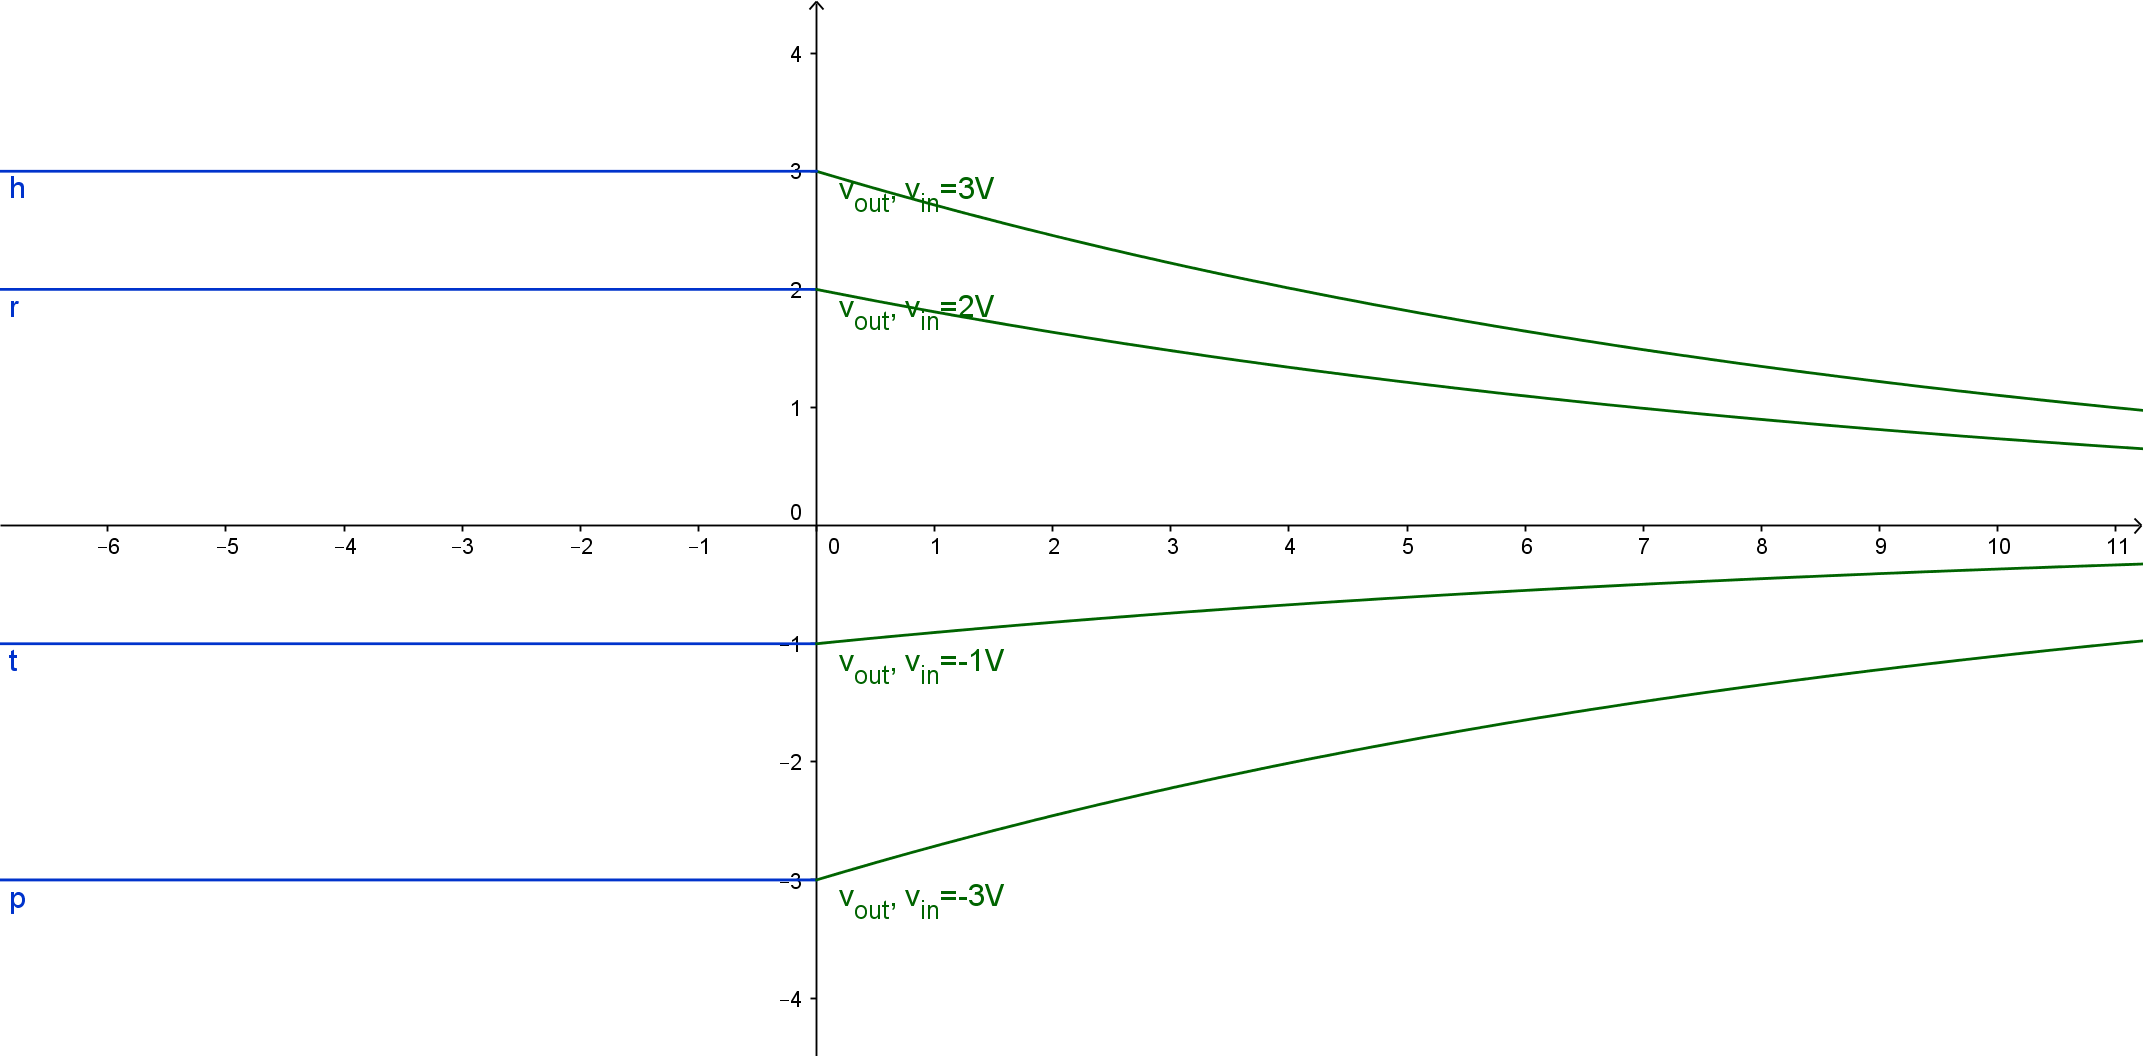
\includegraphics[width=\linewidth]{introduzione/rc_plot}
				\caption{grafico di $v_{out}$}
				\label{graph:rc}
			\end{subfigure}
		\end{figure}
		Supponiamo che: 
		\[
			\begin{cases}
				v_{in}\neq0 \mbox{ se } t<0\\
				v_{in}=0 \mbox{ se } t\geq0
			\end{cases}
		\]
		
		Per $ t<0 $ la tensione sul condensatore \'e uguale alla tensione applicata dal generatore. Quando per $ t\geq0 $ il generatore viene spento ($ v_{in}=0 $), inizia il processo di scarica e la tensione del condensatore tende a zero.
		
		Quindi la tensione sul condensatore non dipende istantaneamente dalla tensione applicata dal generatore ($ v_{in} $ per $ t>0 $), ma dipende anche dalla condizioni iniziali ($ v_{in}\ \mbox{per}\ t<0$).
		
		Scriviamo le equazioni di questo sistema dinamico:
		\[
			v_R = Ri \quad\Rightarrow\quad i = \dfrac{v_R}{R} = \dfrac{v_{in}-v_{out}}{R} , \quad  \quad
			 v_{in} = v_R + v_{out} , \quad  \quad
			\dot v_{out} = \frac{1}{C}i 
		\]
		Mettendo assieme queste equazioni otteniamo:
		\[ \Rightarrow\quad i = C \cdot v_{out} = \dfrac{v_{in}-v_{out}}{R} \]
		
		La corrente $ i $ \'e una quantit\'a che evolve nel tempo, ma nell'equazione scompare. Si tratta di una variabile interna che pu\'o essere sostituita dalla tensione.
		
		Ridefiniamo alcune variabili:
		\[ v_{in}(t) \triangleq u(t) \qquad v_{out}(t) = y(t) \]
		
		Il sistema pu\'o essere descritto con:
		\begin{itemize}
			\item
				un'equazione differenziale lineare a coefficienti costanti:
				\[
					RC \dot y(t) = u(t) - y(t) \quad \quad
					\Rightarrow\quad  \dot y(t) + \dfrac{1}{RC} y = \dfrac{1}{RC} u
				\]
				
				$ R $ e $ C $ sono due parametri che per\'o sono sempre uniti nell'equazione del sistema. Infatti $ RC $ \'e la costante di tempo $ \tau $.
			\item
				la funzione di trasferimento:
				\[ T(s) = \dfrac{\dfrac{1}{RC}}{s+\frac{1}{RC}} = \dfrac{1}{1+s\tau} \] 
			\item
				equazione di stato:
				\begin{align*}
					x(t) &\triangleq y(t)\\
					\dot x(t) &= -\dfrac{1}{RC} x(t) + \dfrac{1}{RC} u(t)
				\end{align*}
				$ x(t) $ \'e la variabile di stato e in questo caso coincide con l'uscita del sistema.
		\end{itemize}
		
		
	\section{Variabili di un sistema}
			\begin{figure}[H]
				\centering
				\includegraphics[width=.3\textwidth]{introduzione/sistema}
			\end{figure}
			\begin{itemize}
				\item ingressi regolabili $ \underline u(t) $
				\item ingressi non regolabili o disturbi $ \underline d(t) $
				\item parametri $ \theta $: non impongono cambiamenti al sistema ma ne modificano la configurazione.
				\item variabili interne o variabili di stato $ \underline x(t) $: sono variabili che vengono descritte dall'evoluzione del sistema secondo leggi definite.
				\item uscite $ \underline y(t) $
			\end{itemize}
		
	\section{Sistemi non lineari}
		Finora abbiamo studiato esempi di sistemi lineari descritti da equazioni lineari. Nel mondo fisico per\'o praticamente tutti i sistemi sono non lineari.
		
	\subsection{Massa-molla}
		\begin{figure}[H]
		\centering
		\begin{subfigure}[b]{0.4\linewidth}
			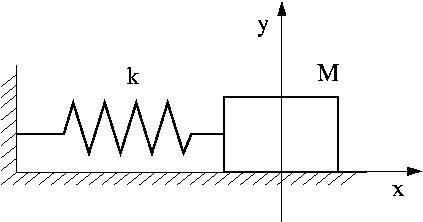
\includegraphics[width=.8\linewidth]{introduzione/massa_molla}
			\caption{$F_{el}(t)=-kx(t)$}
		\end{subfigure}
		\quad \quad
		\begin{subfigure}[b]{0.4\linewidth}
			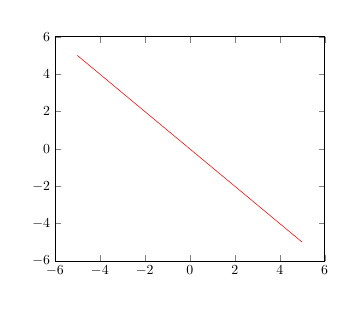
\begin{tikzpicture}[scale=.5]
			\begin{axis}
			\addplot[color=red]{-x};
			\end{axis}
			\end{tikzpicture}
			\caption{$F_{el}(t)=-kx(t)$}
		\end{subfigure}
		\end{figure}
		\'E un modello che descrive la forza elastica, ma non completamente.\\
		Infatti la molla ha una struttura fisica: anche se applichiamo una forza sempre maggiore, la molla raggiunge la sua lunghezza minima (completamente compressa). Quindi la forza elastica diventa una forza vincolare.\\
		Questo modello matematico non considera i casi limite nei quali si perde la linearit\'a.\\
		Quindi i modelli matematici che descrivono le leggi fisiche attraverso i sistemi lineari sono solo approssimazioni per "piccole variazioni''.
		
	\subsection{Vasca}
		\begin{figure}[H]
		\centering
		\includegraphics[width=.3\textwidth]{introduzione/vasca}
		\end{figure}
		\[
			\begin{cases}
				h(t) & \quad \text{altezza colonna $H_{2}O$} \quad (h(t)>0)\\
				u(t) & \quad \text{portata in ingresso}\\
				l(t) & \quad \text{portata in uscita}\\
				E & \quad \text{sezione foro uscita della vasca}\\
				S & \quad \text{sezione della vasca (costante su tutta l'altezza)}
			\end{cases}
		\]
		u(t) \'e l'ingresso che possiamo controllare attraverso un rubinetto.\\
		l(t) e h(t) sono entrambe possibili uscite, ma scegliamo $y(t) \equiv h(t)$ perch\'e \'e misurabile pi\'u facilmente. Infatti non \'e detto che le uscite siano sempre misurabili.\\
		Modelliamo il sistema:
		\begin{equation}
			S \dot{h(t)} = u(t) - l(t)
		\end{equation}
		dove $S \dot{h(t)}$ rappresenta la variazione di volume rispetto al tempo.\\
		Inoltre non conosciamo $l(t)$ e dobbiamo ricavarlo: consideriamo una particella d'acqua che scende dalla cima della vasca fino all'uscita inferiore e calcoliamone il bilancio energetico.
		\[
			\not{m} gh = \frac{1}{2} \not{m} v^2 \; \rightarrow \;
			gh = \frac{1}{2} v^2 \; \rightarrow \;
			v(t) = \sqrt{2gh(t)} \; \rightarrow \;
			l(t) = E \sqrt{2gh(t)} \; \rightarrow \;
			S \dot{h(t)} = u(t) - E \sqrt{2gh(t)}
		\]
		\begin{equation} \label{eq.vasca_non_lineare}
			\dot{h(t)} = - \frac{E}{S} \sqrt{2g} \sqrt{h(t)} + \frac{1}{S} u(t)
		\end{equation}
		Poich\'e la derivata dell'uscita non \'e una combinazione lineare degli ingressi, questa \'e un'equazione differenziale non lineare.\\
		Inoltre esistono dei vincoli fisici che in questa equazione non vengono considerati: 
		\(
			\begin{cases}
				0 \leq h(t) \leq h_{max}\\
				0 \leq u(t) \leq u_{max}
			\end{cases}
		\)
		Infatti anche se $h(t)$ diventa maggiore dell'altezza massima della vasca, l'equazione del modello dice che la variazione di altezza cresce (se supponiamo il secondo membro di \ref{eq.vasca_non_lineare}), mentre in realt\'a si dovrebbe annullare.
		
	\section{Linearizzazione}
		Consideriamo il sistema della vasca nel paragrafo precedente: fissiamo un altezza $ \bar{h} $ e supponiamo che $u(t) \equiv \bar{u} = e \sqrt{2g \bar{h}}$. Ne segue che $ \dot{h}(\bar{t}) =0 $.\\
		Questa situazione \'e detta condizione di equilibrio e $( \bar{h} , \bar{u}) $ \'e il punto di equilibrio.\\
		Riscriviamo l'equazione \ref{eq.vasca_non_lineare}:
		\[ \dot{h(t)} = f(h(t),u(t)) \]
		Adesso calcoliamo l'approssimazione di Taylor fino al primo ordine intorno a \( (\bar{h},\bar{u}) \) :
		\[
			f(h(t),u(t)) = f(\bar{h},\bar{u}) + \left. \frac{\partial f(h,u)}{\partial h} \right|_{(\bar{h},\bar{u})} (h(t) - \bar{h}) + \left. \frac{\partial f(h,u)}{\partial u} \right|_{(\bar{h},\bar{u})} (u(t) - \bar{u}) + \mbox{Resto}
		\]
		poich\'e $ f(\bar{h},\bar{u}) =0$\\
		\[
			\left. \frac{\partial f(h,u)}{\partial h} \right|_{(\bar{h},\bar{u})} = - \frac{E}{2S} \sqrt{2g} \left. \frac{1}{\sqrt{h}} \right|_{(\bar{h},\bar{u})} = - \frac{E}{2S} \sqrt{\frac{2g}{\bar{h}}} = - \alpha \quad (\alpha > 0)\]
			\\
		\[
			\left. \frac{\partial f(h,u)}{\partial u} \right|_{(\bar{h},\bar{u})} = \frac{1}{S} = \beta \quad (\beta > 0)  
		\]
		Definiamo:
		\[ \delta h(t) \triangleq h(t)- \bar{h} \quad \text{la variazione di $h$ rispetto al punto di equilibrio;} \]
		\[ \delta u(t) \triangleq u(t)- \bar{u} \quad \text{la variazione di $u$ rispetto al punto di equilibrio;} \]
		Se $u(t)$ \'e vicino a $\bar{u}$, allora $\delta u(t)$ pu\'o essere negativo purch\'e $u(t)>0$. Analogamente vale per $h(t)$.\\
		Calcoliamo la derivata assoluta rispetto al tempo della variazione di altezza:
		\[ \delta \dot{h(t)} = \frac{\mathrm{d}}{\mathrm{d} t}(h(t)-\bar{h}) = \frac{\mathrm{d}}{\mathrm{d} t}h(t) \doteq \dot{h(t)} \] 
		Abbiamo trovato che la derivata di $h(t)$ e $\delta h(t)$ sono uguali per piccole variazioni.\\
		Quindi in conclusione si ottiene:
		\begin{equation}
			\delta \dot{h(t)} = -\alpha \delta h(t) + \beta \delta u(t)
		\end{equation}
		\'E sensato modellare la vasca come un sistema lineare, ma solo se stiamo lavorando con piccole variazioni rispetto ad un punto di equilibrio.
\end{document}